% universal settings
\documentclass[12pt,twoside,onecolumn,openany,extrafontsizes,dvipsnames]{memoir}

\usepackage[utf8]{inputenc}
\usepackage[T1]{fontenc}
\usepackage{graphicx}


%%%%%%%%%% BOOK INFORMATION %%%%%%%%%%
\newcommand{\authorname}{Michal Chovanec, PhD.}
\newcommand{\booktitle}{Motoko Ice Dragon X}
\newcommand{\subtitle}{Documentation}
\newcommand{\publisher}{Publisher}
\newcommand{\editionyear}{2024}
\title{\booktitle}
\author{\authorname}


\begin{document}

\chapter{Hardware description}
%\section{block diagram}

\newpage

\begin{figure}[h]
    
    \includegraphics[scale=0.28]{../images/schem.png}
    \caption{schematic diagram of DC motor version}
\end{figure}


\newpage

\begin{figure}[h]
    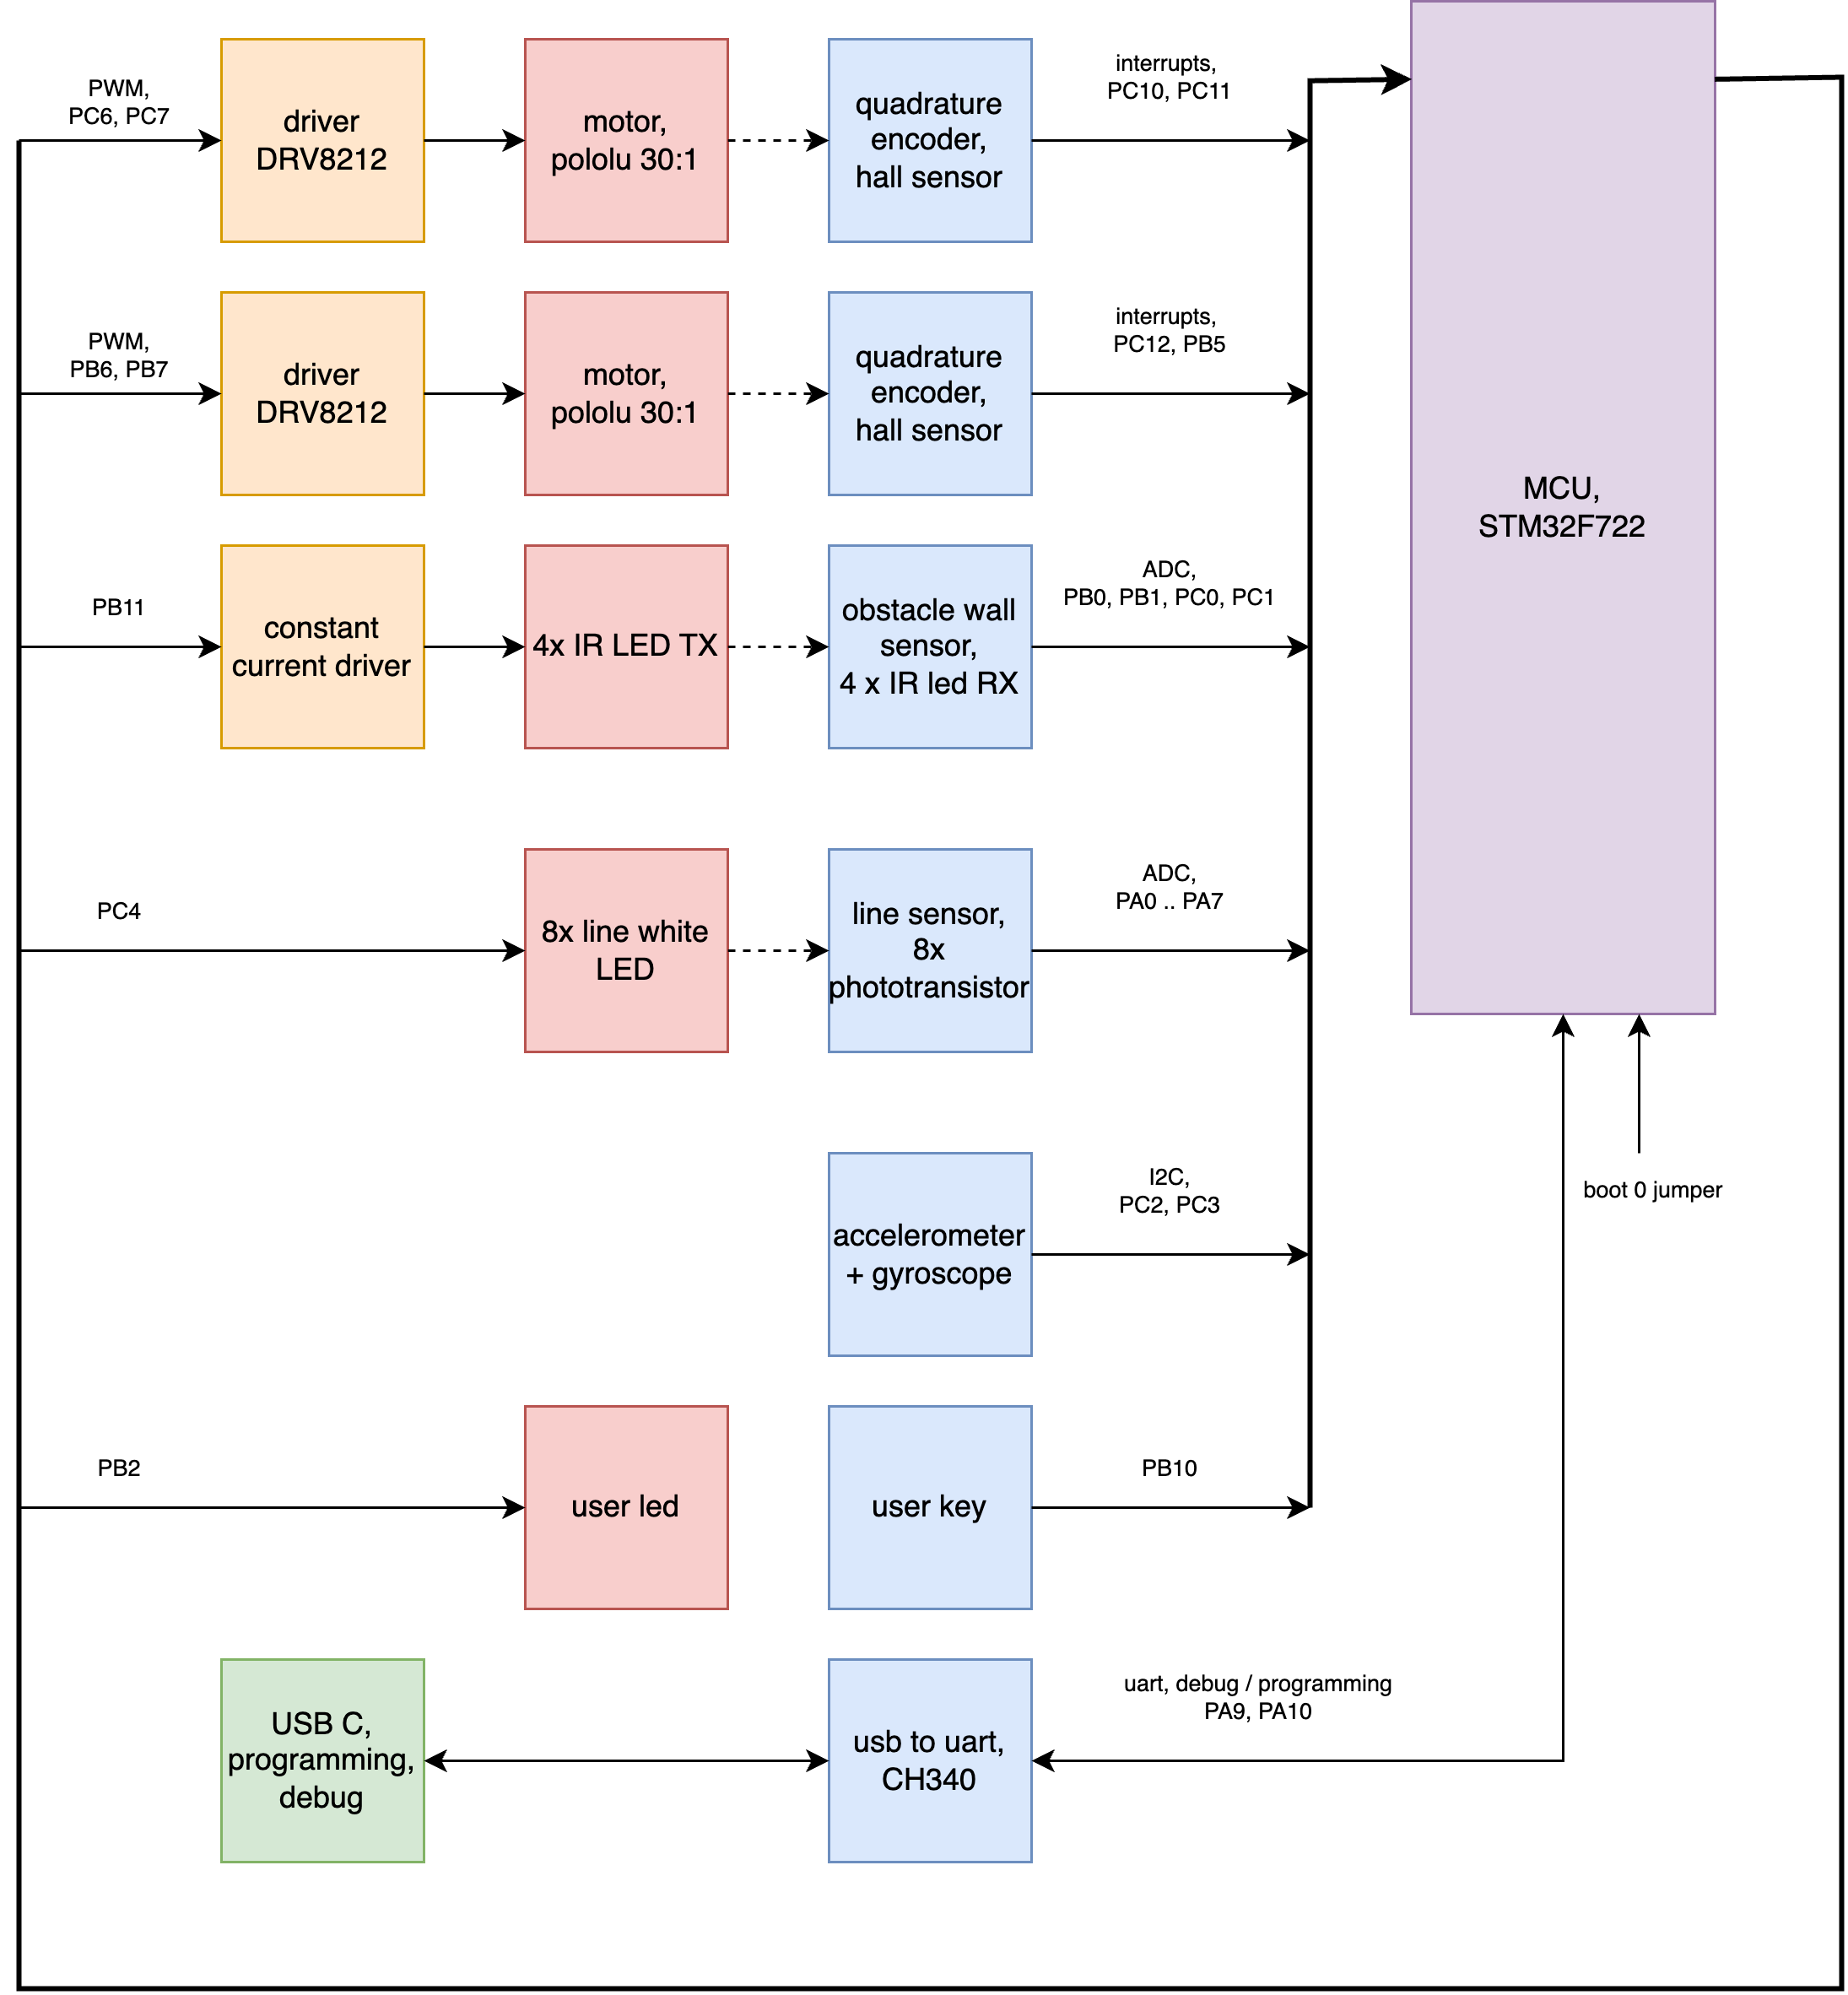
\includegraphics[scale=0.8]{../diagrams/diagrams.png}
    \caption{block diagram of DC motor version}
\end{figure}


\newpage

    \begin{table}[h!]
        \centering
            \begin{tabular}{||c c c c c||} 
            \hline
            pin number & pin name & function & peripheral & AF number \\
            \hline\hline
                14 & PA0 & line sensor ADC0, right & ADC1 & N/A \\ 
                15 & PA1 & line sensor ADC1 & ADC1 & N/A \\ 
                16 & PA2 & line sensor ADC2 & ADC1 & N/A \\ 
                17 & PA3 & line sensor ADC3 & ADC1 & N/A \\ 
                20 & PA4 & line sensor ADC4 & ADC1 & N/A \\ 
                21 & PA5 & line sensor ADC5 & ADC1 & N/A \\ 
                22 & PA6 & line sensor ADC6 & ADC1 & N/A \\ 
                23 & PA7 & line sensor ADC7, left & ADC1 & N/A \\ 
                & & & & \\
                25 & PB0 & IR sensor ADC8, front left  & ADC1 & N/A \\ 
                26 & PB1 & IR sensor ADC9, left & ADC1 & N/A \\ 
                8 & PC0 & IR sensor ADC10, right & ADC1 & N/A \\ 
                9 & PC1 & IR sensor ADC11, front right & ADC1 & N/A \\ 
                & & & & \\
                51 & PC10 & encoder left A  & GPIO & N/A \\ 
                52 & PC11 & encoder left B  & GPIO & N/A \\ 
                53 & PC12 & encoder right A  & GPIO & N/A \\ 
                57 & PB5  & encoder right B  & GPIO & N/A \\ 
                & & & & \\
                37 & PC6 & PWM left A   & TIM 150 & N/A \\ 
                38 & PC7 & PWM left B   & TIM & N/A \\ 
                58 & PB6 & PWM right A  & TIM & N/A \\ 
                59 & PB7 & PWM right B  & TIM & N/A \\ 
                & & & & \\
                10 & PC2 & IMU I2C, SDA & GPIO & N/A \\ 
                11 & PC3 & IMU I2C, SCL & GPIO & N/A \\ 
                & & & & \\
                42 & PA9 & uart TX & UART1 & N/A \\ 
                43 & PA10 & uart RX & UART1 & N/A \\ 
                & & & & \\
                27 & PB2 & user LED & GPIO & N/A \\ 
                28 & PB10 & user Key & GPIO & N/A \\ 
                29 & PB11 & IR led control & GPIO & N/A \\ 
                24 & PC4 & line led control & GPIO & N/A \\ 
                & & & & \\
                7 & NRST & reset &  &  \\ 
                60 & BOOT0 & firmware bootloader control &  &  \\ 
            \hline
            \end{tabular}
        \caption{pin mapping and function}
        \label{table:1}
    \end{table}


\end{document}